\chapter{Ressonadors electromagnètics}

\section{Introducció}

Un ressonador és bàsicament una caixa de la que les ones no poden eixir, acumulant-se l' energia. Les ones interferiran amb les seues reflexions a les parets, pel que certes freqüències tenen ressonància. Aquest fenomen té moltes aplicacions: filtres freqüencials, emmagatzematge d' energia, forns de microones, acceleradors de partícules...

\section{Paràmetres d' un ressonador}

\begin{wrapfigure}{r}{7cm}
 % \centering
  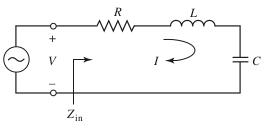
\includegraphics[scale=0.5]{RLCres}
  \caption{Circuit RCL equivalent}
  \label{RCLc}
\end{wrapfigure}

Un ressonador pot modelar-se com un circuit RCL (figura \cref{RCLc}), i està caracteritzat per els paràmetres d' aquest: la resistència, la inducció, la capacitat i el voltatge d' entrada.

La corrent d' aquest circuit és
\begin{equation}
  I_g = \frac{V_g}{R + \jmath \left (L \omega - \frac{1}{c\omega} \right)}
\end{equation}
Coneixent aquests paràmetres podem obtindre la potència generada (que és la mateixa dissipada per la resistència):
\begin{equation}
  P_g = P_R = \frac{1}{2}R \abs{I} ^2 = \frac{\frac{1}{2} R \abs{ V_g} ^2}{R^2 + \left(L \omega - \frac{1}{c\omega} \right)^2}
  \label{potg}
\end{equation}

\subsection{Freqüència de ressonància}

La corba de \cref{potg} és alta per a freqüències al voltant d' un valor $\omega _0$ que fa que el denominador siga mínim:
\begin{equation}
L \omega_0 - \frac{1}{C\omega _0} = 0 \to \omega _0 = \frac{1}{\sqrt{LC}}
\end{equation}

i baixa per a freqüències allunyades d' aquest valor, com es mostra a la figura \cref{potplot}.

\begin{figure}[ht]
  \centering
  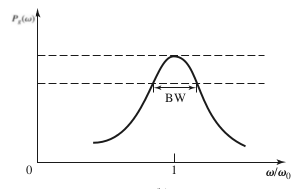
\includegraphics[scale=0.5]{poweroutput}
  \caption{Potència d' eixida d' un generador}
  \label{potplot}
\end{figure} 

L' amplada d' aquesta corba està caracteritzada pel factor de qualitat $Q$, definit com a 
\begin{equation}
  Q = \frac{\omega _ 0 }{\omega _2 - \omega _1}
\end{equation}

per a $\omega_2 > \omega _1$ tal que
\begin{equation}
P_g(\omega_2) = P_g (\omega _1 ) = \frac{1}{2} P_max = \frac{1}{2} \left ( \frac{1}{2} \frac{\abs{V_g} ^2}{R} \right ) 
\end{equation}

Quan més alt és $Q$ més selectiu és el filtre (menor ample de banda $BW$). Si resolem

\begin{equation}
P_g(\omega) = \frac{1}{2} P_max \to \frac{1}{4}\frac{\abs{V_g} ^2}{R} = \frac{\frac{1}{2} R \abs{ V_g} ^2}{R^2 + \left(L \omega - \frac{1}{c\omega} \right)^2}
\end{equation}
arribem al valor aproximat 
\begin{equation}
  (\omega - \omega_0) \sim \pm \frac{1}{2}\frac{R}{L} \to 
  \left\{ 
  \begin{array}{lr}
    \omega _2 = \omega _0 + \frac{1}{2}\frac{R}{L} \\
    \omega _1 = \omega _0 - \frac{1}{2}\frac{R}{L} 
  \end{array}
  \right.
\end{equation}

Pel que $\omega_2 - \omega_1 = \frac{R}{L}$ i $Q = \frac{\omega _0}{\omega_2 \omega _1} = \omega _0 \frac{L}{R} = \sqrt{\frac{L}{C}}\frac{1}{R}$

\subsection{Energia emmagatzemada}

La inductància i el condensador del circuit emmagatzemen energia, mentre que la resistència en perd. El quocient entre la energia emmagatzemada i la perduda és
\begin{equation}
  \frac{E_{emm}}{E_{per}} = \frac{\langle \frac{1}{2} L \abs{I} ^2 \rangle + \langle \frac{1}{2} C \abs{V} ^2 }{\frac{1}{2} R \abs{I} ^2} \rangle = \frac{\frac{1}{2} \frac{1}{2} L \abs{I} ^2  + \frac{1}{2} \frac{1}{2} C \abs{V} ^2 }{\frac{1}{2} R \abs{I} ^2} = \frac{L \abs{I} ^2 + C \frac{\abs{I}^2}{C^2 \omega^2}}{2 R \abs{I} ^2}
\end{equation}

On $\langle \cdot \rangle$ indica mitjana temporal. En el cas $\omega = \omega _0$ aquest coeficient és $\frac{L}{R}$, i vegem, i comparant-lo amb el factor de qualitat $Q = \omega _0 \frac{L}{R}$ descobrim que aquest també ens informa de la qualitat del ressonador com a emmagatzemador d' energia.

\subsection{Càlcul de Q en guies}

Per a calcular el factor $Q$ d' una guia d' ones usant $Q = \omega _0 \frac{\epsilon(\omega _0)}{P_l(\omega_0)}$ si coneixem la seua freqüència de ressonància $\omega _0$, la energia emmagatzemada $E_{stored} (\omega_0)$ i la potència perduda $P_{lost} (\omega _0)$. Aquesta última pot separa-se en dos contribucions: les pèrdues del conductor $P_{l,cond}$ i les del dielètric $P_{l,diel}$, i fer:
\begin{equation}
Q = \omega _0 \frac{E_s}{P_{l,c} + P_{l,d}} = \left [ \frac{P_{l`c}}{\omega_0 E_s }+\frac{P_{l`c}}{\omega _0 E_s} \right ] ^{-1} = \left [ \frac{1}{Q_D }+\frac{1}{Q_C} \right ] ^{-1}
\end{equation}

\subsubsection*{$Q$ d' un dielèctric}

La energia emmagatzemada en un dielèctric, en funció dels camps magnètics al seu interior, és
\begin{equation}
E_s = E_s(\vec E) + E_S(\vec H) = \frac{1}{2}\frac{1}{2} \int \vec E \cdot \vec D ^{*} dV + \frac{1}{2}\frac{1}{2} \int \vec H \vec B ^{*}dV = \frac{1}{2} \int \vec E \cdot \vec D^{*} dV = \frac{1}{2} \int \vec H \vec B ^{*} dV
\end{equation}

On hem utilitzat que en camps no atenuats la energia emmagatzemada pels camps elèctrics i magnètics és la mateixa. La potència perduda és
\begin{equation}
P_{l`d} = \frac{1}{2} \int \vec E \cdot \vec J ^{*} dV = \frac{\sigma_D}{2} \int \vec E \cdot \vec E ^{*} dV
\end{equation}
I per tant el factor $Q$ és
\begin{equation}
  Q_D = \omega _0 \frac{E_S}{P_l} = \frac{\frac{1}{2} \sigma _D \int \abs {\vec E} ^2 dV}{\frac{1}{2} \epsilon_0 \epsilon _r \int \abs{\vec E} ^2 dV} = \omega _0 \frac{\sigma _D}{\epsilon _0 \epsilon _r} = \frac{1}{tg\delta}
\end{equation}

\subsubsection*{$Q$ d' un conductor}

La $Q$ d' un conductor not pot calcular-se en general, ja que la potència perduda és
\begin{equation}
  P_l = \frac{1}{2} R_S \int _{parets} \abs{\vec H} ^2 d \vec S
\end{equation}
i no podem trobar-la si desconeixem les parets.

\section{Cavitats ressonants}

\subsection{Cavitat paral·lelepipèdica}

Considerem una paral·lelepípede de material conductor en el que existeix el mode $TM_{mn}$ (figura \cref{rectres}). Els curtcircuits (si el considerem com una guia rectangular curtcircuitada) provoquen reflexions que donen a una ona $+$ cap a $+x$ i una ona $-$ cap a $-x$. Els camps d' aquests modes ja els hem obtés en \cref{rectTM}. Per comoditat els reescrivim agrupant factors en els coeficients $\bar{e_i ^+}$:

\begin{figure}[ht]
  \centering
  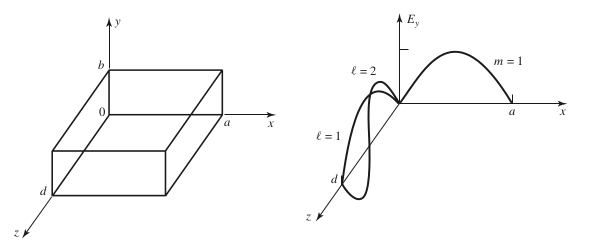
\includegraphics[scale=0.5]{rectres}
  \caption{Ressonador paral·lelepipèdic i els seus camps ressonants }
  \label{rectres}
\end{figure}

\begin{equation}
  \nonumber
  \begin{array}{ccc}
    e_z^+  = E_0 ^+ \bar{e_z ^+} & e_x^+ = E_0 ^+ \bar {e_x ^+} & e_y ^+ = E_0 ^+ \bar{e_y ^+} \\
    h_z ^+ = 0 & h_x ^+ = E_0 ^+ \bar {h_x ^+} & h_y^ + = E_0 ^+ \bar {h_x ^+} \\ 
  \end{array}
\end{equation}

Els camps de la ona $-$ só iguals però canviant $\beta \to -\beta$ i $H_0 ^+ \to H_0 ^-$. En termes dels coeficients  $\bar{e_i ^+}$ queden:
 
\begin{equation}
  \nonumber
  \begin{array}{ccc}
    e_z ^- =  E_0 ^- \bar{e_z ^+} & e_x ^- = -E_0 ^- \bar {e_x ^+} & e_y ^- = -E_0 ^- \bar{e_y ^+} \\
    h_z ^- =  0 & h_x ^- =  E_0 ^- \bar {h_x ^+} & h_y ^- =  E_0 ^- \bar {h_x ^+} \\
  \end{array}
\end{equation}

per a la $-$. Sumant aquestes expressions obtenim les interferències:
\begin{subequations}
  \begin{align}
    E_z &= E_0 ^+ \bar{ e_z ^+} \e{-\jmath \beta z} + E_0 ^- \bar{ e_z ^+} \e{\jmath \beta z} \\
    E_x &= E_0 ^+ \bar{ e_x ^+} \e{-\jmath \beta z} - E_0 ^- \bar{ e_x ^+} \e{\jmath \beta z}  \\
    E_y &= E_0 ^+ \bar{ e_y ^+} \e{-\jmath \beta z} - E_0 ^- \bar{ e_y ^+} \e{\jmath \beta z}  \\    
    H_z &= 0 \\
    H_x &= E_0 ^+ \bar{ h_x ^+} \e{-\jmath \beta z} + E_0 ^- \bar{ h_x ^+} \e{\jmath \beta z}  \\
    H_y &= E_0 ^+ \bar{ h_y ^+} \e{-\jmath \beta z} + E_0 ^- \bar{ h_y ^+} \e{\jmath \beta z} 
  \end{align}
\end{subequations}

Apliquem les condicions de contorn:
\begin{enumerate}
  \item{$E_x (z=0) = 0 \to \bar{e_x ^+} ( E_o ^+ \e{-0} - E_o ^- \e{0}) = 0 \to E_0 ^+ = E_0 ^- $}
  \item{$E_x (z=c) = 0 \to \bar{e_x ^ +} E_0 ^+ ( \e{- \jmath \beta c} - \e{\jmath \beta c}) = 0 \to \sin \beta c = 0 \to \beta c = l \pi$ amb $l \in \Zahl$}
\end{enumerate}

Les freqüències d' aquestes ones són les de ressonància:
\begin{equation}
 \beta ^2 =  \omega ^ 2 \mu \epsilon - \left ( \frac{n \pi}{a} \right ) - \left ( \frac{m \pi}{b} \right ) = \left ( \frac{l\pi}{c} \right ) ^2 \to  \omega _{mnl} = \frac{1}{\sqrt{\mu \epsilon}} \sqrt{ \left ( \frac{n \pi}{a} \right ) + \left ( \frac{m \pi}{b} \right ) + \left ( \frac{l \pi}{c} \right )}
\end{equation}

\subsubsection{Cavitat circular}

Per a trobar les freqüències de ressonància d' una guia circular curtcircuitada (figura \cref{circres}) procedim com abans: escrivim els camps dels modes $TE_{mn}$ en direcció $+z$ i $-z$, els sumem i apliquem les condicions de contorn $E_{\varphi}(z=0) = E_s (z=0) = 0$ i $E_{\varphi}(z=c) = E_s (z=c) = 0$, i obtenim la restricció per a $\beta$, que és la mateixa d' abans: $\beta c = l \pi$ amb $l \in \Zahl$. 

\begin{figure}[ht]
  \centering
  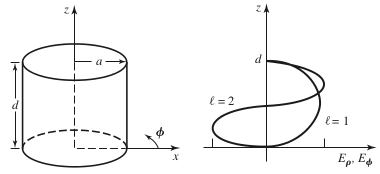
\includegraphics[scale=0.5]{circres}
  \caption{Ressonador paral·lelepipèdic i els seus camps ressonants }
  \label{circres}
\end{figure}

Les freqüències de ressonància són per tant 

\begin{equation}
  \beta ^2 = \omega ^2 \mu \epsilon - \left ( \frac{P_{mn}}{a} \right ) ^2 = \left ( \frac{l\pi}{c} \right ) \to \omega _{mnl} = \sqrt{\left ( \frac{P_{nm}}{a} \right ) ^2 + \left ( \frac{n}{c} \right ) ^2 }
\end{equation}
